% VLDB template version of 2020-08-03 enhances the ACM template, version 1.7.0:
% https://www.acm.org/publications/proceedings-template
% The ACM Latex guide provides further information about the ACM template

\documentclass[sigconf, nonacm]{acmart}

%% The following content must be adapted for the final version
% paper-specific
\newcommand\vldbdoi{XX.XX/XXX.XX}
\newcommand\vldbpages{XXX-XXX}
% issue-specific
\newcommand\vldbvolume{14}
\newcommand\vldbissue{1}
\newcommand\vldbyear{2020}
% should be fine as it is
\newcommand\vldbauthors{\authors}
\newcommand\vldbtitle{\shorttitle} 
% leave empty if no availability url should be set
\newcommand\vldbavailabilityurl{http://vldb.org/pvldb/format_vol14.html}
% whether page numbers should be shown or not, use 'plain' for review versions, 'empty' for camera ready
\newcommand\vldbpagestyle{plain} 



\usepackage{stfloats}


\begin{document}
\title{A Survey on Join Algorithms Using MapReduce}

%%
%% The "author" command and its associated commands are used to define the authors and their affiliations.
\author{Chenhao Fang}
\affiliation{%
  \institution{University of Wisconsin - Madison}
  \streetaddress{1423 Monroe Street}
  \city{Madison}
  \state{Wisconsin}
  \postcode{53711}
}
\email{cfang45@wisc.edu}



%%
%% The abstract is a short summary of the work to be presented in the
%% article.
\begin{abstract}
The popular MapReduce framework is widely used to analyze and process large amount of data. In this work, we present a survey on join algorithms using the MapReduce framework. Join operation is one of the most important and time consuming operations in Database Management Systems. Many research are trying to propose new join algorithms using MapReduce environment. We talk about the MapReduce system and execution process of it. We review the state-of-art algorithms for both two-way and multi-way join algorithms and compare them on several important metrics. We also present analysis of them and discussion about their limitations. This survey can help researchers study the difference of join algorithms in a chronological manner. Concluding, we talk about the direction for future work on join algorithms using MapReduce.
\end{abstract}

\maketitle

%%% do not modify the following VLDB block %%
%%% VLDB block start %%%
\pagestyle{\vldbpagestyle}
\begingroup\small\noindent\raggedright\textbf{PVLDB Reference Format:}\\
\vldbauthors. \vldbtitle. PVLDB, \vldbvolume(\vldbissue): \vldbpages, \vldbyear.\\
\href{https://doi.org/\vldbdoi}{doi:\vldbdoi}
\endgroup
\begingroup
\renewcommand\thefootnote{}\footnote{\noindent
This work is licensed under the Creative Commons BY-NC-ND 4.0 International License. Visit \url{https://creativecommons.org/licenses/by-nc-nd/4.0/} to view a copy of this license. For any use beyond those covered by this license, obtain permission by emailing \href{mailto:info@vldb.org}{info@vldb.org}. Copyright is held by the owner/author(s). Publication rights licensed to the VLDB Endowment. \\
\raggedright Proceedings of the VLDB Endowment, Vol. \vldbvolume, No. \vldbissue\ %
ISSN 2150-8097. \\
\href{https://doi.org/\vldbdoi}{doi:\vldbdoi} \\
}\addtocounter{footnote}{-1}\endgroup
%%% VLDB block end %%%



\section{Introduction}

The big data and distributing computing is drawing many attentions from both researchers or industries. With the development of new technologies like LoT, AI, cloud computing services and web apps, the amount of data generated every day is at an unprecedented rate.  The MapReduce framework was first introduced by Google in \cite{62}. In this programming model and framework for data processing, the details of parallel execution is hided and users are allowed to only focus on data processing strategies. 

Join operation is one of the most important and time consuming operations in Database Management Systems. Therefore, many research are trying to improve the join operation in MapReduce environment using different methods and techniques. In this paper, we will first talk about the MapReduce framework and execution process of MapReduce. Then, we will survey researchers works on join algorithms using MapReduce based on the type of join algorithms using a chronological manner: Map-Side Joins, Reduce-Side Joins, Filter-Based Joins, MapReduce variants and so on. Then, we will analysis and compare them. We summarize the results in a table for quick reference. In the end, we will present our future work about survey and experiments in the future. 

This paper is organized as follows: In section 2, we will talk about the background about MapReduce framework and related work. From section 3 to section 7, we will present five categories of join algorithms using MapReduce and make comparison on them. Section 8 and 9 presents the conclusion and proposes future work
\section{Background}

\subsection{MapReduce Overview}
The MapReduce was first introduced by Jeff Dean and Sanjay Ghemawat in \cite{62}. It is a programming model and the framework implementation that supports the model for processing and generating large data sets. In this programming model, the details of parallel execution is hided and users are allowed to only focus on data processing strategies. Users only need to specify a \textit{map} function that can process a key-value pair and produce a set of intermediate key/value pairs, and a \textit{reduce} function that merges all the intermediate values associated with the same intermediate key. Users can define their own \textit{map} and \textit{reduce} function based on their own requirements. Some examples that can be implemented easily in MapReduce are: Distributed Grep, Count of URL Access Frequency, Reverse Web-Link Graph, Term-Vector per Host, Inverted Index and Distributed Sort. These examples are discussed in detail in Jeff's original paper.

\subsection{Execution}
In Jeff and Sanjay's paper
\cite{62}, the overall flow of a MapReduce operation in Google's implementation is explained in details. They were shown in \autoref{fig:1}.

\begin{figure}
  \centering
  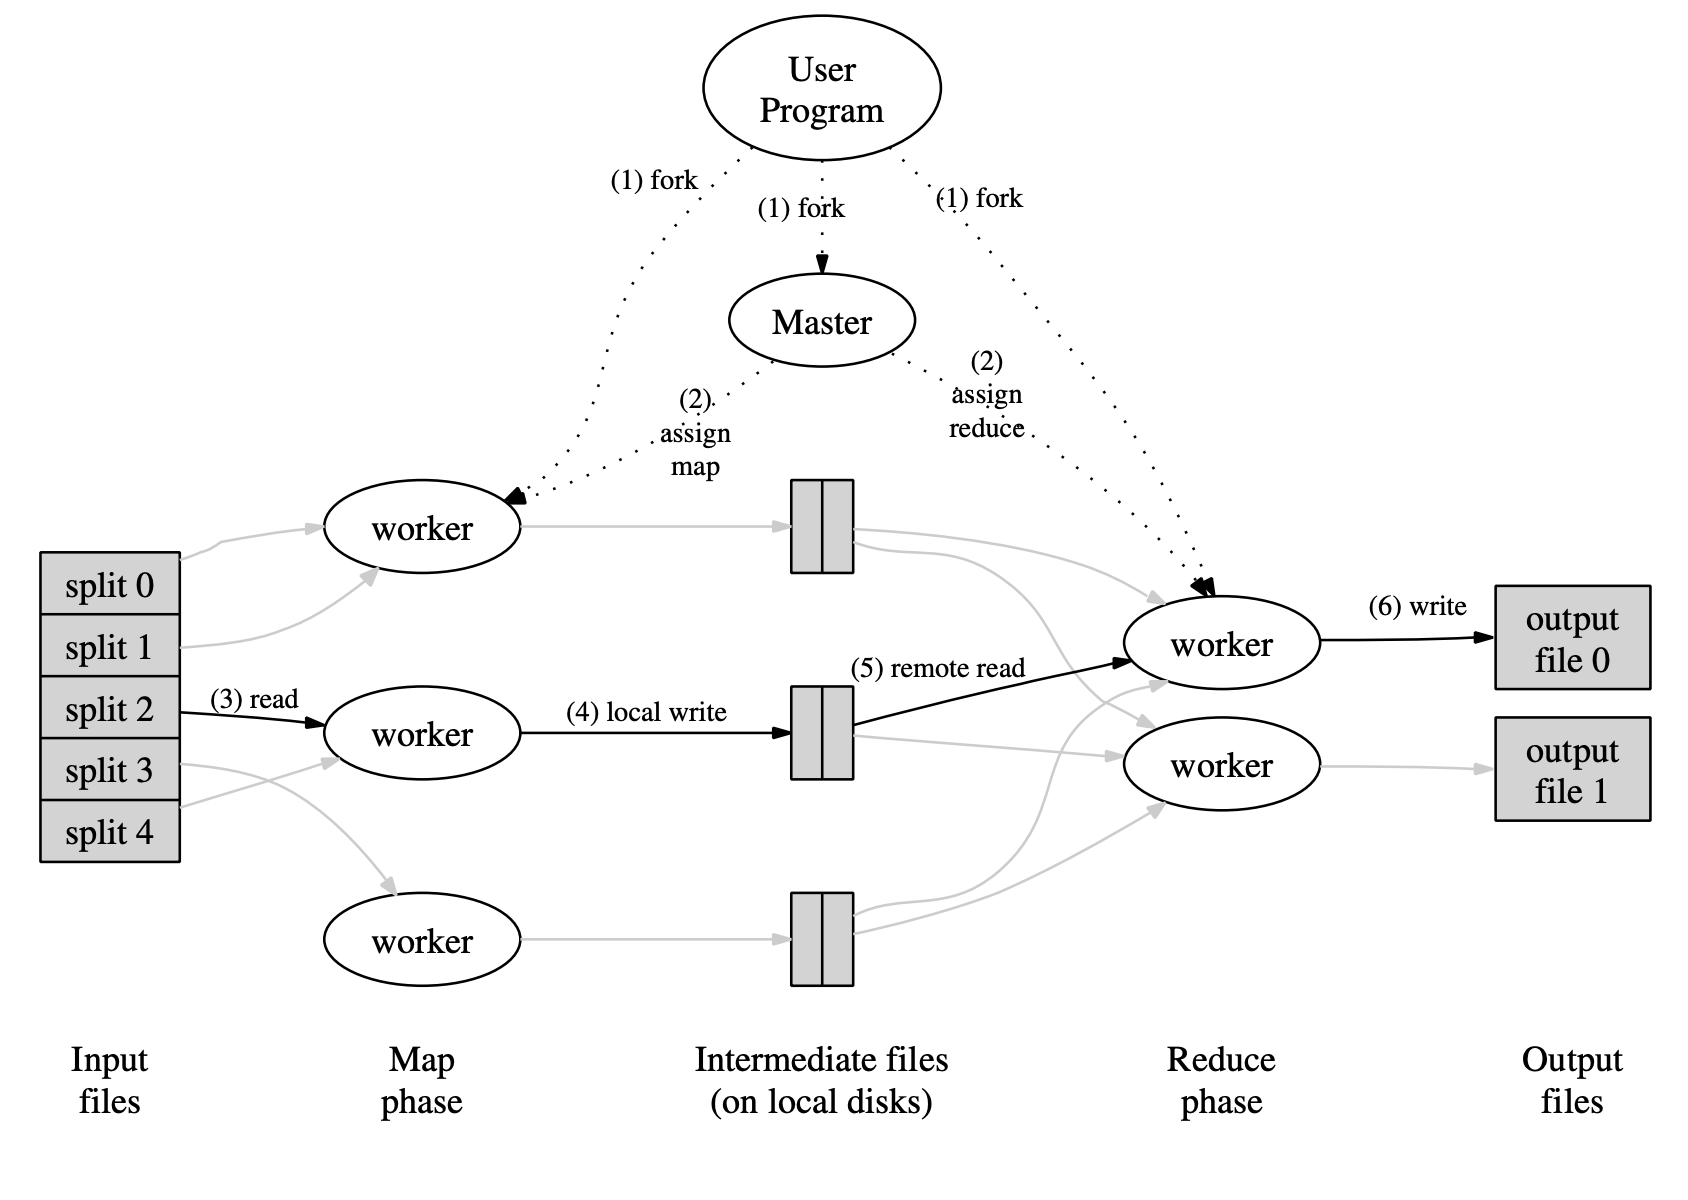
\includegraphics[width=\linewidth]{figures/1.png}
  \caption{Execution overview of MapReduce.  Figure from Jeffery Dean, \textit{MapReduce: Simplified Data Processing on Large Clusters}, 2004.}
  \label{fig:1}
\end{figure}

If the user calls the MapReduce function, the following procedure happens(The numbers in \autoref{fig:1} correspond to the numbers below):

\begin{enumerate}
    \item The user-defined MapReduce program will be split by the MapReduce library into M pieces. The size of each piece can be controlled by user. 
    
    \item The master node is a special node in MapReduce systems. The master node assigns Map or Reduce work to each worker nodes.
    
    \item The workers who got the Map job read the corresponding input split file. It parse the key-value pairs in the input split file and pass them to the user-defined Map function. After this process, the intermediate key-value pairs are stored in buffer. 
    
    \item The key-value pairs in the buffer are written to disk periodically. They will be partitioned into \textit{R} parts by partitioning function. The master node will send the locations of these pairs in local disks to the workers who have reduce work.
    
    \item The reduce workers will read the buffered data from the local disks. In order to group all the same key together, a reduce work need to sort the intermediate key. However, if the size of intermediate data is too large to fit into memory, the reduce worker will use external sort.
    
    \item The reduce workers will iterate the sorted data and pass the key and the corresponding set of values to user-defined Reduce function. Then the output of user-defined Reduce function will be appended to a output file for this specific partition.
    
    \item When all tasks are completed, the master node will wake up the user program and return back to user code.
\end{enumerate}

Note that the \textit{R} output files do not need to be combined by the user. The reason is that they will usually be passed to another MapReduce call or use then in some other distributed application which can handle multiple files as input.

\subsection{Advantages}

The MapReduce is a simple and easy to use model and framework. The major advantages of MapReduce framework for data processing are listed below:

\subsubsection{\textbf{Simple}} 

The MapReduce is extremely easy to use compared with other distributed processing systems. Users only need to define their own Map and Reduce functions and do not need to consider physical distribution of work and execution plans.

\subsubsection{\textbf{Storage Independent}}

When using MapReduce, you don't need to worry about the underlying storage. The MapReduce is basically independent from storage layers. It can work on different storages like BigTable \cite{27898} and so on.

\subsubsection{\textbf{Flexible}} 

The MapReduce framework and model does not dependencies on data model and schema. Therefore, users can easily deal with unstructured data than traditional Database Management Systems.

\subsubsection{\textbf{Scalability}}

The MapReduce framework has a very high scalability. This is MapReduce's best advantage. 4 years after the publication time of Jeff's paper \cite{62}, Yahoo!'s Hadoop gear could scale out more than 4000 nodes.


\subsection{Related Work}
In Blanas \cite{blanas2010comparison}, they provided detailed description and implementation of several join algorithms using the MapReduce framework. For each algorithm, they designed practical pre-processing techniques to improve the performance. Later, they conducted experiments evaluation to compare the different join algorithms on Hadoop cluster. Their work shows the tradeoffs among different join algorithms and the benefits of using MapReduce to process join.

In Lee\cite{lee2012parallel}, they provided different technical aspects about the MapReduce framework and classified and summarized works on pros and cons of using MapReduce for data processing. Moreover, the optimization of MapReduce was reviewed. They roughly classified join algorithms into Map-Side Joins and Reduce-Side Joins.

In a paper published in 2020 by Amer\cite{al2020analysis}, they study two-way join algorithms in MapReduce throughly. They reviewed state of the art two-way join algorithms in MapReduce. They classified two-way join algorithms into four categories: standard equal-joins, filter-based joins, skew insensitive and MapReduce variants. They summarized their advantages and disadvantages so that the users can choose the most suitable two-way join algorithms in their application.

\section{Map-Side Join}

\subsection{Map-Merge Join}

The default implementation of map-side join in Hadoop is Map-Merge Join\cite{lee2012parallel}. It is the most common map-side join and works similarly to the sort-merge join in traditional Database Management Systems. There are three phases in Map-Merge Join where the first and second phases are full MapReduce jobs. The \autoref{fig:2} shows an example of Map-Merge Join. 

\begin{figure*}[h!]
  \centering
  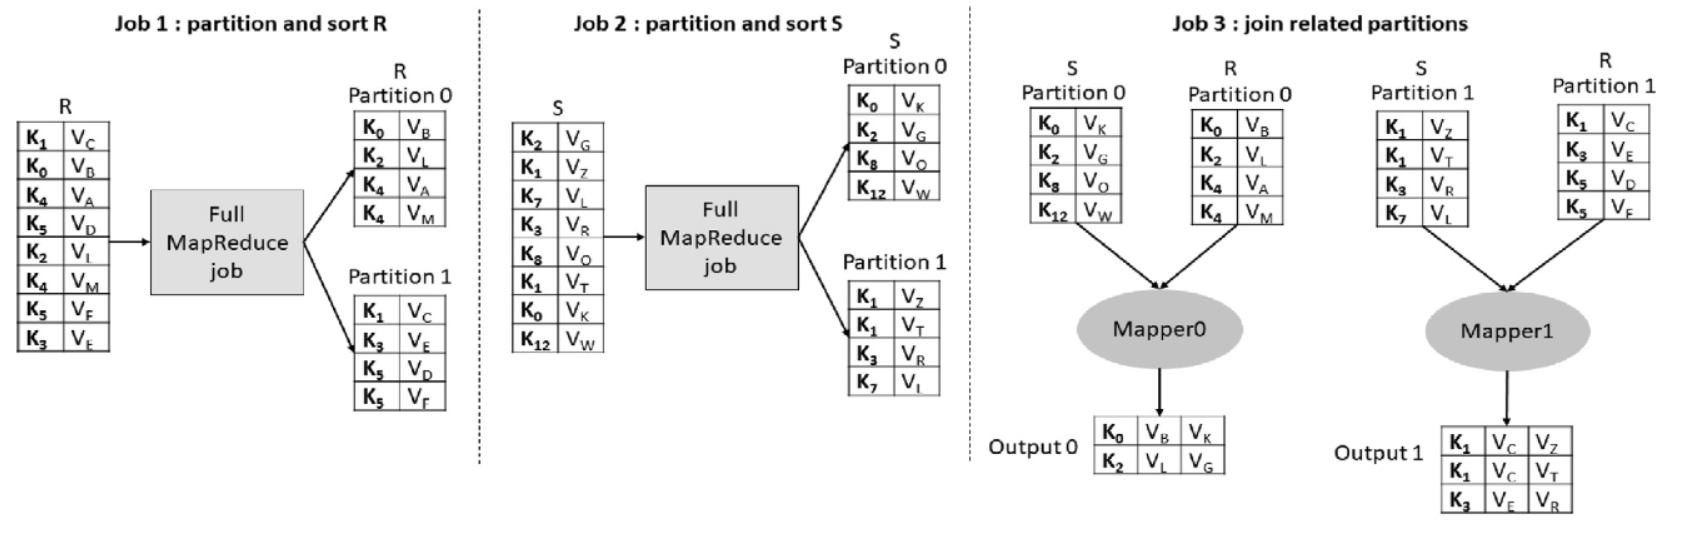
\includegraphics[width=\linewidth]{figures/2.png}
  \caption{An example of Map-Merge Join.  Figure from Amer F. Al-Badarneh, \textit{An analysis of two-way equi-join algorithms under MapReduce}, 2020.}
  \label{fig:2}
\end{figure*}

In the first phase, the relation R is partitioned and sorted on the join keys, so does relation S in the second phase. In the third phase, mappers read the input partitions and merge them. If the input relations are partitioned and sorted in advance, the third phase can be implemented easily. However, if they are not partitioned and sorted, the overall performance of Map-Merge Join will be degraded.



\subsection{Improvements of Map-Merge Join}

The Map-Side Partition Merge Join\cite{pigul2012comparative} is an improvement of the Map-Merge Join algorithm. The name of this algorithm is quite long and the abbreviation is MSPMJ.  It uses on-demand scanning of the second relation and therefore can avoid memory overflow. However, it has the same problem as the Map-Merge Join, which is its ancestor. There are suited for large relation joins, but if at least one of the relations can fit into the node's buffer or cache, they are not optimal. 

\subsection{Map-Side Replication Join}

Given the talk above, the Map-Side Replication Join came out and became the optimal solution \cite{andreas2010designing}. The Map-Side Replication Join is a map-only join algorithm. The \autoref{fig:3} shows the process of Fragment Replicate Join.


\begin{figure}[H]
  \centering
  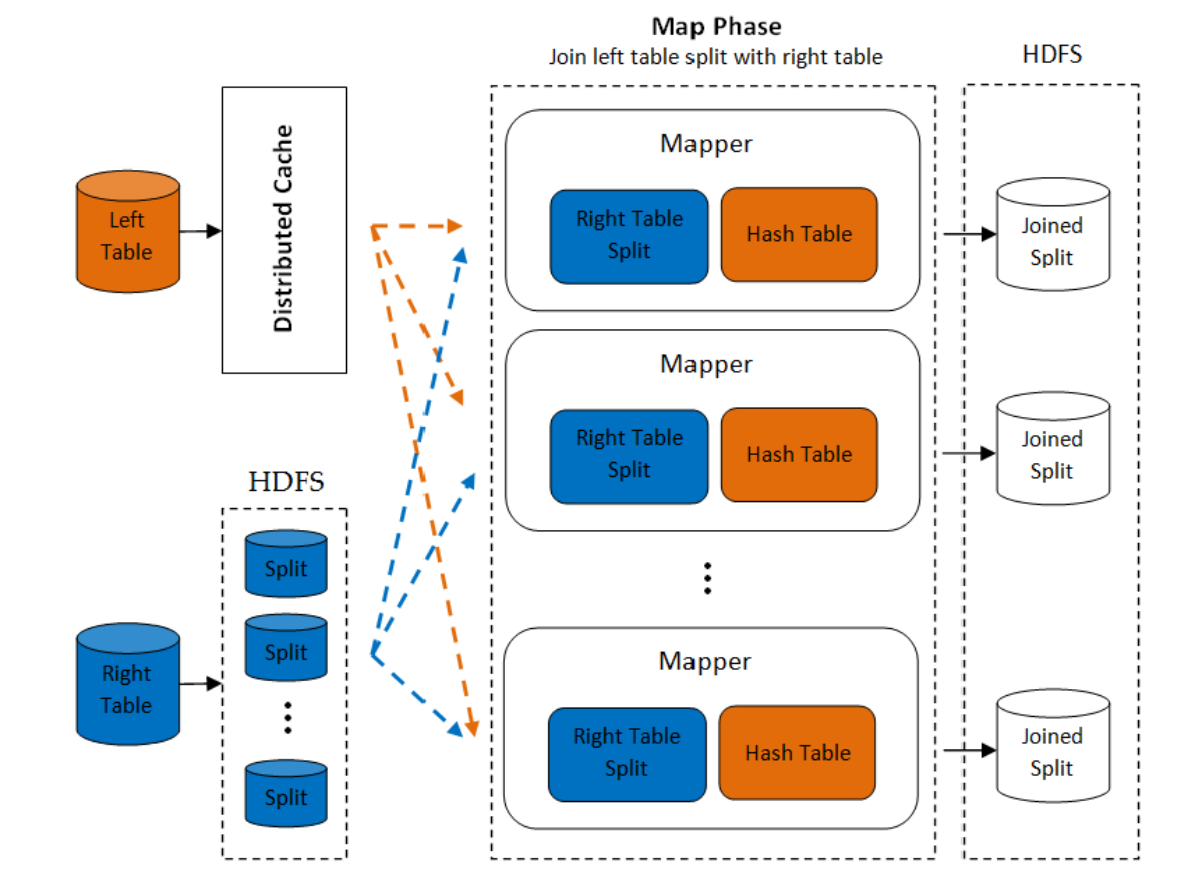
\includegraphics[width=\linewidth]{figures/3.png}
  \caption{Fragment Replicate Join Implementation.  Figure from C. Andreas, \textit{Designing a Parallel Query Engine over Map/Reduce}, 2010.}
  \label{fig:3}
\end{figure}

Consider the left relation L and right relation R, in this case, the size of R is greatly bigger than L. First, the small relation L is replicated into all nodes by using the distributed cache and before the mapper phase, transform it to a hash table. Then for each value in the hash table,  the map phase nest an array list to store rows that has the same join key. For each row of the bigger table, search over the unique keys  of the small table in hash table. If there's a match, write it to the HDFS output. 

However, the Map-Side Partition Merge Join can only be performed if one relation can fit into a node's memory. To improve this, several improved algorithms were proposed, like Reversed Map Join \cite{luo2010adaptive} and Broadcast Join \cite{blanas2010comparison}.

\subsection{Improvements of Map-Side Replication Join}

The Reversed Map Join were first introduced by Luo and Dong in 2010 \cite{luo2010adaptive}. In map phase, the Reversed Map Join builds hash table for each input split of left relation. After that, it iterates through each row of right relation and probes a hash table for each key. Finally, it produces the join result and writes it to the HDFS output. 

The Broadcast Join is a combination of the Map-Side Replication Join and the Reversed Map Join. The smaller left relation is broadcast to each mapper in the map phase and kept in each node's memory. It uses hash table to store the smaller relation and find matches by hash table lookup from the other relation. This algorithm avoids I/Os for moving. Also, there's no need to sorting on both relation. 

\subsection{Comparison}
In this subsection, we provide an analysis of different Map-Side Join algorithms based on several different metrics that can affect overall performance in \autoref{tab:1} 


\begin{table*}[t]
  \caption{Comparison of Map-Side Join}
  \label{tab:1}
  \begin{tabular}{|c|c|c|c|c|l|}
    \toprule
    Algorithms & Supported Join & Pre-processing &  Partitioning & Pros & Cons\\
    \hline\hline
    Map-Merge Join & Multi-way  & Sorting & Hash-based & Easy to implement & Need pre-processing \& Sensitive to data skew \\
    \hline
    MSPMJ & Multi-way & Sorting & Hash-based & Avoid memory overflow & Need pre-processing \& Sensitive to data skew\\
    \hline
    MS Replication Join & Two-way & No & Broadcast & Handle data skew & Has strong condition on relation sizes\\
    \hline
    Reversed Map Join & Two-way & No & Broadcast & Handle data skew & Complex \\
    \hline
    Broadcast Join & Two-way & No & Broadcast & Handle data skew & Perform badly if input increases\\
    
    \bottomrule
  \end{tabular}
\end{table*}


\section{Reduce-Side Join}

\subsection{Standard Repartition Join}
Though Map-Side Join algorithms are easy to implement, the Reduce-Side join are the most common join algorithms when talking about join algorithms in MapReduce. The Standard Repartition Join is the most general Reduce-Side Join algorithms. The Apache Hadoop framework use this algorithm as default implementation. Also, it is widely used in big data systems like Pig, Hive and so on today.  This algorithm only run one MapReduce job. One example of Standard Repartition Join is shown in \autoref{fig:4}.

\begin{figure}[h]
  \centering
  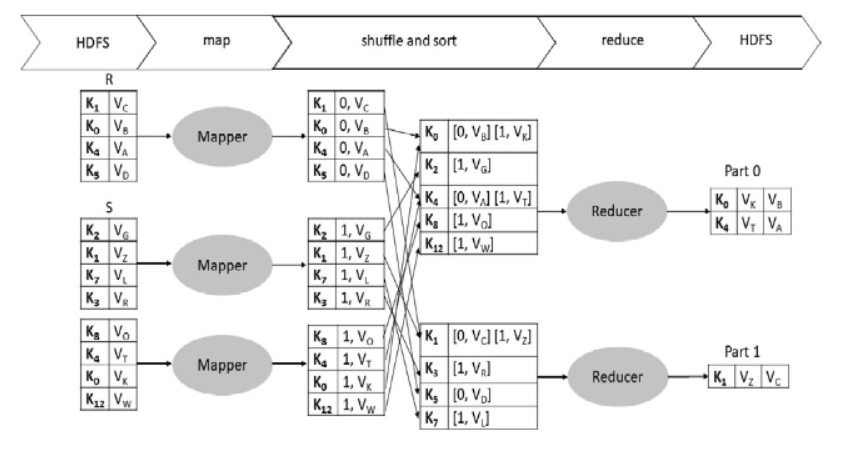
\includegraphics[width=\linewidth]{figures/4.png}
  \caption{An example of Standard Repartition Join.  Figure from Amer F. Al-Badarneh, \textit{An analysis of two-way equi-join algorithms under MapReduce}, 2020.}
  \label{fig:4}
\end{figure}

The special part of this join algorithm is that each mapper will tag each row of relations to identify which relation the row come from. After tagging, the rows that have the same key value are moved to the same reduce node during shuffle and sort phase. And finally, each reduce node will joins the rows which have the same value. This algorithm is similar to the hash join algorithm in traditional Database Management Systems.

However, thought there's no pre-processing requirements nor special treatments in Standard Repartition Join, it has some drawbacks. It requires extra processing time and may lead to network bottleneck.

\subsection{Improved Repartition Join}

In order to improve the performance of the Standard Repartition Join, Blanas\cite{blanas2010comparison} proposed a new method called Improved Repartition Join. The major different between these two methods are the following three: First, in the map phase, the Improved Repartition Join will be a composition of key and the relation tag. Here, the relation tag will ensures records from Right Relation will sorted ahead of records from Left Relation on any given key. The second one is that the hash function is designed in a way that it will only use the join key in the composite key so that the same join key will still be assigned to the same reduce task. Thirdly, due to the reason in the first point, the records that come from Right Relation will be ahead of those from Left Relation. Therefore, only the Right Relation need to be buffered and Left Relation will be streaming data. 

\subsection{"Schimmy" Reduce-Side Join}
Lin proposed a "schimmy" schema to save I/0 cost during the process of reduce-side join. \cite{lin2010data} In this method, the messages are separated from graph structure data. It will only shuffle the message to save the cost of shuffling data. The mappers only need to emit messages and reducers read graph structure data from HDFS directly. After these processes, do a reduce-side merge join between the data and messages to perform join.

\subsection{Comparison}
The comparison of different Reduce-Side Join algorithms based on several different metrics are shown in  \autoref{tab:3} 


\begin{table*}[hbt!]
  \caption{Comparison of Reduce-Side Join}
  \label{tab:3}
  \begin{tabular}{|c|c|c|c|c|l|}
    \toprule
    Algorithms & Supported Join & Pre-processing &  Partitioning & Pros & Cons\\
    \hline\hline
    Standard RJ & Multi-way  & No & Hash-based & No size restriction & Memory overflow \& Sensitive to data skew \\
    \hline
    Improved RJ & Multi-way & No & No & Fix buffering problem above & Sensitive to data skew\\
    \hline
    "schimmy" RJ & Two-way & Graph data & No & Save I/O cost & Need complex preprocessing\\
    
    \bottomrule
  \end{tabular}
\end{table*}

\section{Filter-Based Join}
\subsection{Semi-Join}
In real application, if the Right relation is extremely large, many of its records may not be matched by records from Left relation. A semi-join might be used here to avoid sending unused rows of R over the network. 

The semi-join were first implemented by Blanas\cite{blanas2010comparison}. This method contains three phases with each phase corresponding to a single MapReduce job. The figure \ref{fig:5} shows an example of semi-join. 

\begin{figure*}[hbt!]
  \centering
  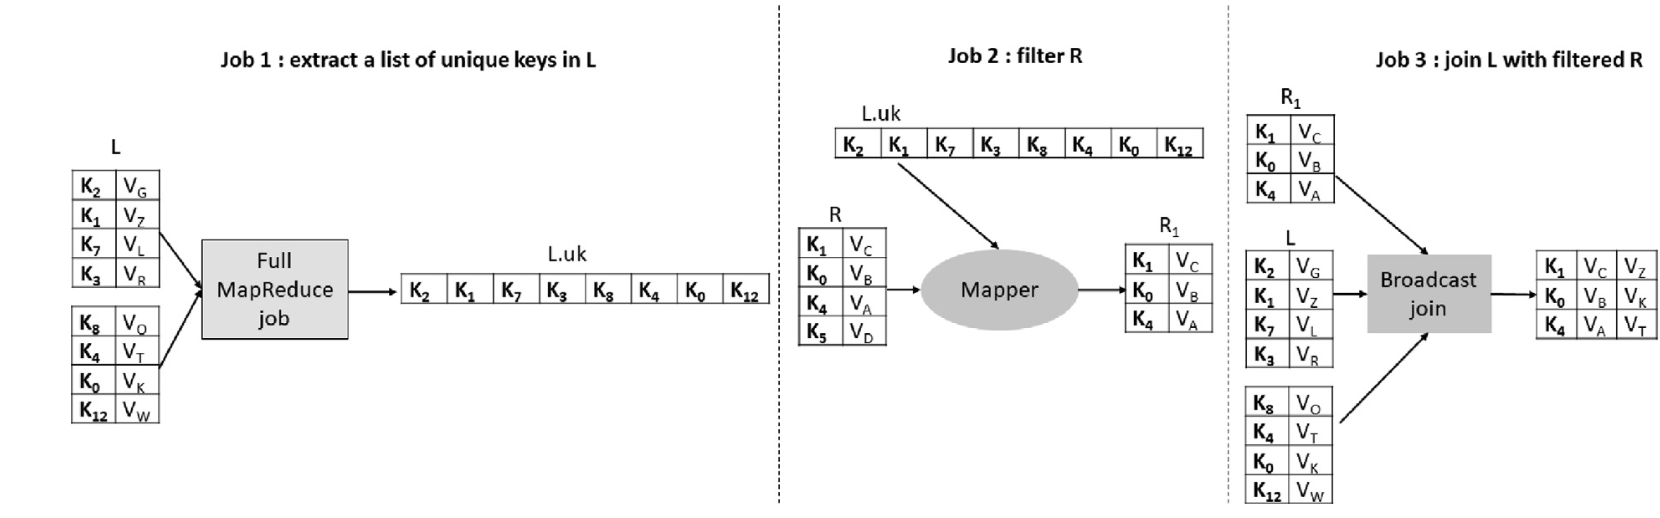
\includegraphics[width=\linewidth]{figures/5.png}
  \caption{An example of Semi-Join.  Figure from Amer F. Al-Badarneh, \textit{An analysis of two-way equi-join algorithms under MapReduce}, 2020.}
  \label{fig:5}
\end{figure*}

The first phase will build a hash table to determine all the unique join keys of Left relation. Then, one reduce node will collect all the unique keys in one file \textit{L.uk}. One assumption is that this file can fit into memory. In the second phase, the \textit{L.uk} will be loaded into a hash table. The mapper will iterate through Right relation and output the record if the key is in \textit{L.uk}. In the third phase, all the split of R will join with L using the broadcast join method described before. 

This semi-join algorithm will reduce the cost of sending unused part of R through network. However, it need to scan an extra round of L. Also, there are still some redundant records in R after the filter that do not join with a particular split of L. This problem can be solved by Per-Split Semi-Join. 

\subsection{Per-Split Semi-Join}

The Per-Split Semi-Join is also proposed by Blanas in the same paper\cite{blanas2010comparison}. This method also has three phases like Semi-Join, with each phase corresponding to one MapReduce job. The first phase generates set of unique keys for every split of $L_i$ and store them in several files $L_i.uk$ In the second phase, R will be loaded to hash table in different split. Each $L_i.uk$ file will match the hash table and output $R_i$. In the third phase, the $R_i$ and $L_i$ will be simply joined by any join method. In the Per-Split Semi-Join, the third phase is extremely easy since the first two phases will do most work. This algorithm can benefit a lot using pre-processing. 

However, both Semi-Join and Per-Split Semi-Join will require three phases and three MapReduce jobs. They need to submit jobs many times and therefore will impact the performance.

\subsection{Hash-and-Position-Based Per-Split Semi-Join}

In 2015, Matono \cite{matono2015improvement} proposed the Hash-and-Position-Based Per-Split Semi-Join to improve the drawback of the above two algorithms. It has a long name, let's just call it HPB PSSJ or HPB. In this method,  the author introduced three new reducers and thus number of MapReduce jobs is reduced to two. The first job contains only map phase. The mapper will create hash table $L_i.hp$ for each split of L with the hash value of the keys and their relative positions. In the second phase, the mapper will create hash table $H_{Ri}$ to store the hash values for each split of R and perform actual join. 

\subsection{Bloom Join}

In Zhang \cite{zhang2013efficient}, the authors proposed a new method of using Bloom filter to join relations in MapReduce. In Bloom Join, the technique is similar to the Semi-Join. They used a Bloom filter based on the R relation to filter part of relation S. In their experiment, the size of both relation R and S is 100 million records.

\subsubsection*{Two-Stage Join} This algorithm contains two stages and two MapReduce jobs. The \autoref{fig:6} shows an example of Two-Stage Bloom Join.

\begin{figure}[hbt!]
  \centering
  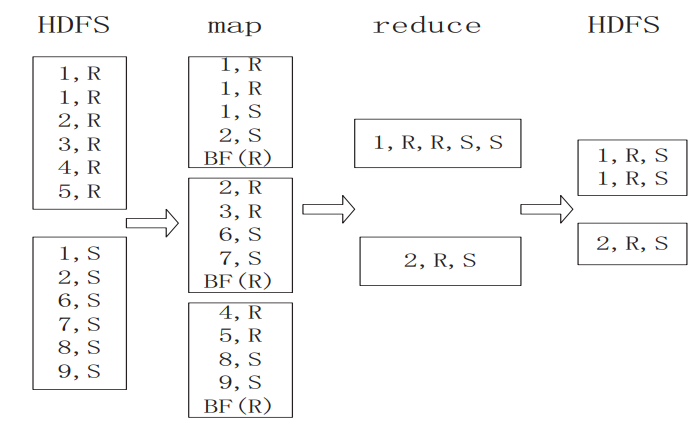
\includegraphics[width=\linewidth]{figures/6.png}
  \caption{An example of Two-Stage Bloom Join  Figure from Zhang, \textit{Efficient Processing Distributed Joins with Bloomfilter
using MapReduce}, 2013.}
  \label{fig:6}
\end{figure}

In the first stage, a Bloom filter is build for relation R. Then the mapper uses the Bloom filter to filter relation S and outputs the key-value pairs of the join key an tagged record. All the records will be sent to reducer and the reducer will separate and buffer the input into two sets and then perform a cross-product. 

\subsubsection*{Three-Stage Join} This algorithm contains three phases and three MapReduce jobs. The \autoref{fig:7} shows an example of Three-Stage Bloom Join.

\begin{figure}[hbt!]
  \centering
  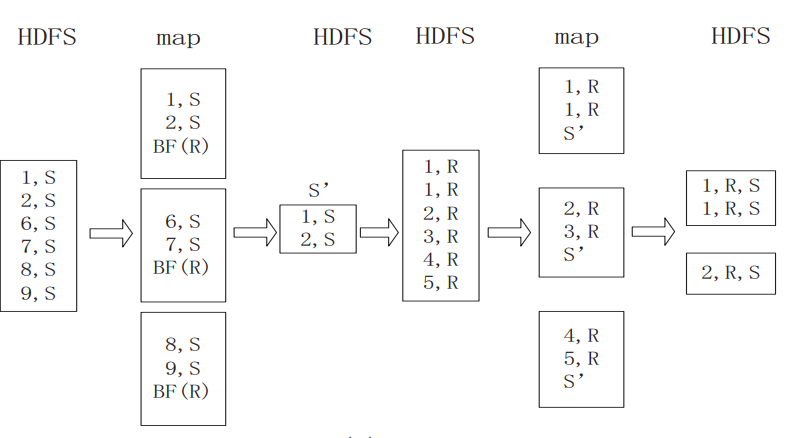
\includegraphics[width=\linewidth]{figures/7.png}
  \caption{An example of Three-Stage Bloom Join  Figure from Zhang, \textit{Efficient Processing Distributed Joins with Bloomfilter
using MapReduce}, 2013.}
  \label{fig:7}
\end{figure}

This first stage is identical to the Two-Stage Join algorithm, while in the second stage, the Bloom filter will be broadcasted to filter S. After this phase, there will be a list of files $S_i$ and they will join with R in the third phase. The jobs in the second and third phase are both map-only jobs.


\subsection{Comparison}

The comparison of different Reduce-Side Join algorithms based on several different metrics are shown in  \autoref{tab:4} 


\begin{table*}[hbt!]
  \caption{Comparison of Filter-Based-Side Join}
  \label{tab:4}
  \begin{tabular}{|c|c|c|c|c|l|}
    \toprule
    Algorithms & Supported Join & Pre-processing &  Partitioning & Pros & Cons\\
    \hline \hline
    Semi-Join & Multi-way  & Filtering & Hash-based & Eliminate redundant records & Inefficient if there are too many keys \\
    \hline
    Per-Split Semi-Join & Multi-way & Filtering & Hash-based & Eliminate redundant records & Complexcity\\
    \hline
    HPB PSSJ & Multi-way & Filtering & Hash-based & Use hash instead of list & More complesx\\
    \hline
    Bloom Join & Two-way & Sorting & No & Space-efficient & Redundant rows in the other table\\
    \hline
    Two-Stage Join  & Two-way & No & Hash-based & Space-efficient & Redundant rows in the other table\\
    \hline
    Three-Stage Join & Two-way & No & Hash-based & Space-efficient & Need three MapReduce jobs\\
    
    \bottomrule
  \end{tabular}
\end{table*}

\section{MapReduce Variants}

There have been several research work on modification of the MapReduce framework to cope with the join process. 

\subsection{Map-Reduce-Merge}

Map-Reduce-Merge is the first attempt to optimize join problems in MapReduce framework\cite{10.1145/1247480.1247602}.To support binary operations including join, the normal Map and Reduce phase in MapReduce framework. In the merge phase, the merger receives the output from two distinguish reduce sources. Then the merge phase processes two key-value pairs and output a new merged key-value pair. The data and control flow of Map-Reduce-Merge framework is shown in \autoref{fig:8}

\begin{figure}[hbt!]
  \centering
  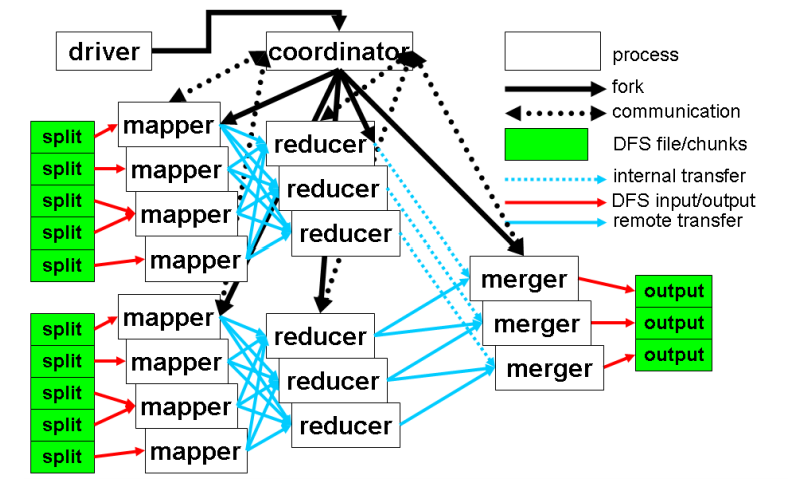
\includegraphics[width=\linewidth]{figures/8.png}
  \caption{Data and control flow for the MapReduce-Merge framework.  Figure from Yang, \textit{Map-Reduce-Merge: Simplified Relational Data Processing on Large Clusters}, 2013.}.
  \label{fig:8}
\end{figure}

This modification retains many advantages of MapReduce, while adding the ability of processing heterogeneous inputs. 

\subsection{Map-Join-Reduce}

Map-Join-Reduce is another variant of MapReduce framework that can perform one-phase join. It adds a join stage before reduce stage. First, every mapper reads records from relations that will be joined. Then, the mapper outputs are shuffled and moved to joiners. The joiners are run inside the reduce nodes.  The joiners will perform actual join operations. 

\subsection{Comparison}

Though MapReduce variants can help the framework improve the ability of data processing, they still require a lot of spaces to store the intermediate results. Also, they need to do modification to a mature framework, therefore, they were not used widely compared with algorithms talked above. 

The comparison of different MapReduce variants are shown in  \autoref{tab:5} 

\begin{table*}[hbt!]
  \caption{Comparison of MapReduce variants}
  \label{tab:5}
  \begin{tabular}{|c|c|c|c|c|l|}
    \toprule
    Algorithms & Supported Join & Pre-processing &  Partitioning & Pros & Cons\\
    \hline \hline
    Map-Reduce-Merge & Two-way  & No & No & Efficient for heterogenous data & Hard to implement \\
    \hline
    Map-Join-Reduce & Two-way & No & No & Efficient for heterogenous data & Hard to implement\\
    \bottomrule
  \end{tabular}
\end{table*}


\section{Other Join Algorithms}

\subsection{Hybrid Hadoop Join}
Atta\cite{atta2010implementation} developed a hybrid approach that is a combination of Map-Side and Reduce-Side join. This algorithm only performs a partial partition-wise join and the join happens in reduce phase. The \autoref{figure:9} shows the dataflow of Hybrid Hadoop Join.

\begin{figure}[hbt!]
  \centering
  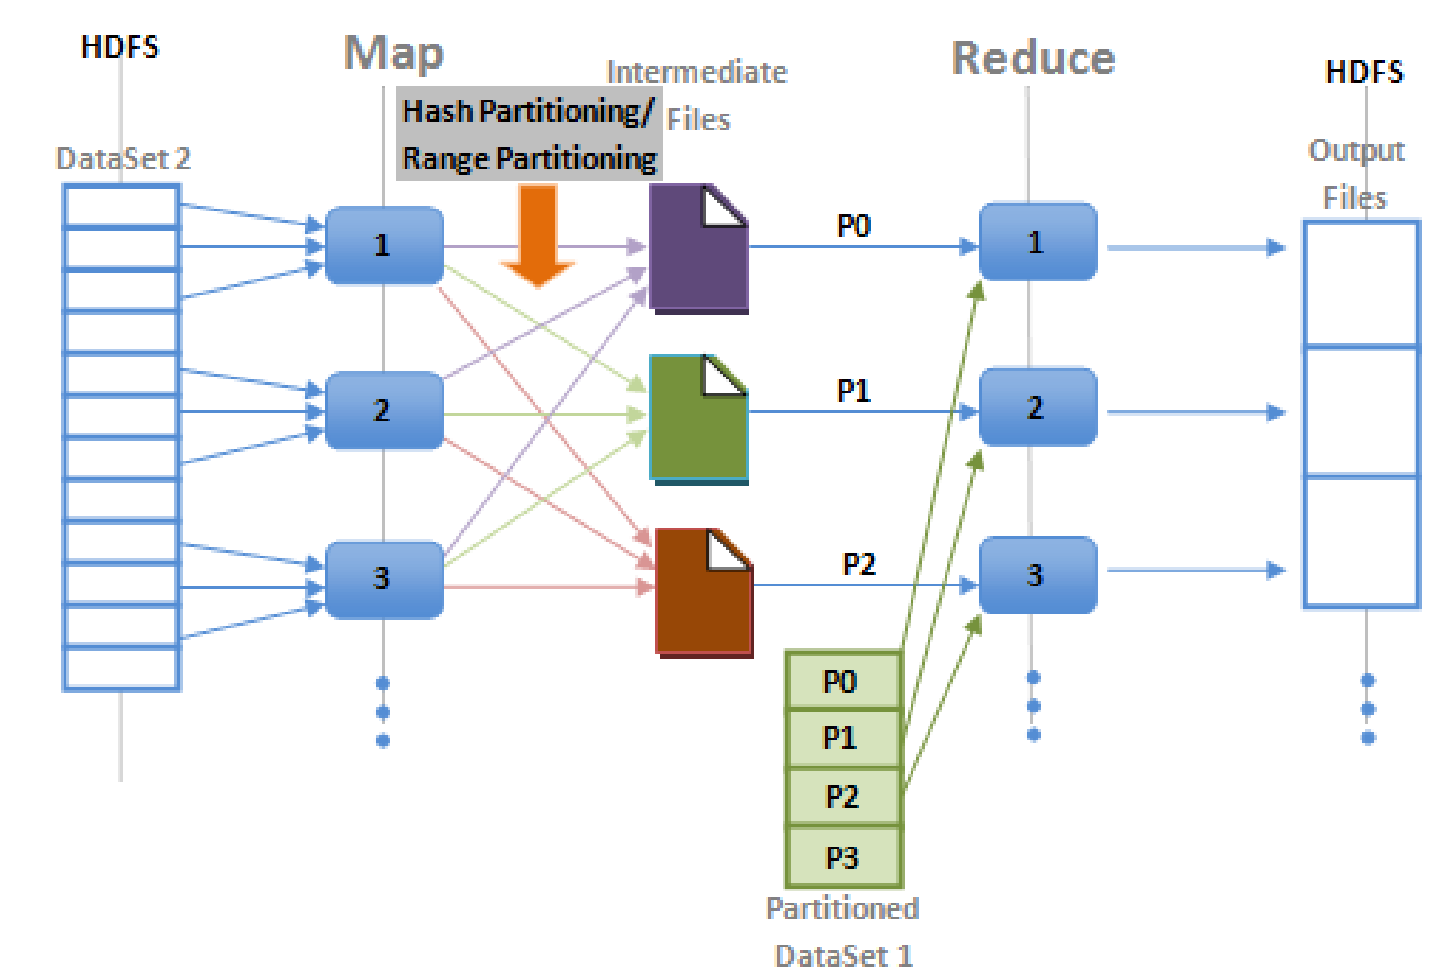
\includegraphics[width=\linewidth]{figures/9.png}
  \caption{Data and control flow for the Hybrid Hadoop framework.  Figure from Atta, \textit{Implementation and Analysis of Join Algorithms to Handle Skew for the Hadoop Map/Reduce Framework.}, 2010.}.
  \label{fig:9}
\end{figure}

The Hybrid Hadoop join has two phases and two MapReduce jobs. In the first job, the algorithm partitions and sorts the smaller relation to different splits $R_i$. Next, in the second job, each mapper will iterate through rows of $R_i$ and pass the key-value pars to the partitioning function. It will partition and sort S in the same way that R was partitioned and sorted. Then the output of partitioning function will be passed to reducers and in each reducer, the counter part of $R_i$ will be loaded into a hash table. Finally, the reducer will probe the hash table for each input key of $S_i$ and perform the join operation. The final output will be written to HDFS. 

This algorithm have the advantage of Map-Side Join and Reduce-Side Join. Moreover, t eliminates the overhead of the tagging, and since only one relation need to be partitioned, it limits the pre-processing. However, it still has drawbacks of the Map-Side Join and Reduce-Side Join. Also, the parameters has to be set properly in this algorithm.


\subsection{Theta Join}
The first Theta Join using MapReduce is first introduced by Okcan\cite{okcan2011processing}. The main idea of this algorithm is to reduce task by partitioning join space, through balancing the input and output cost of reduce jobs. Also, it will minimize the number of input records that are duplicated. This algorithm uses a reducer-centered cost model that can calculate the total cost of cross product of mapper output. Using this model, it just assigns the mapper output to reducers that can minimize the job running time. 

\subsection{Comparison}
The comparison between these two algorithms are shown in \autoref{tab:6}.

\begin{table*}[hbt!]
  \caption{Comparison of MapReduce variants}
  \label{tab:6}
  \begin{tabular}{|c|c|c|c|c|l|}
    \toprule
    Algorithms & Supported Join & Pre-processing &  Partitioning & Pros & Cons\\
    \hline \hline
    Hybrid Hadoop Join & Multi-way  & sorting & Hash-based & Less prerequisites & Complex \\
    \hline
    Theta Join & Multi-way & No & No & Minimize running time & Need partitioning and replication\\
    \bottomrule
  \end{tabular}
\end{table*}

\section{Conclusion}
The join operation is the most important and costly operation in Database Management Systems. In this survey, we reviewed several state of the art join algorithms in MapReduce framework and compared them using several important metrics. We first discussed the MapReduce system and its methodology. The core of this work is surveying on five different kinds of join algorithms: Map-Side Join, Reduce-Side Join, Filter-Based Join, MapReduce Variants and other types. We hope this work will help researchers compare different join algorithms using MapReduce easily when they are trying to propose new improvements or new ideas in this area.

In the future work, we will research on other join algorithms and different join conditions like Similarity Join, KNN Join, Top-K Join and so on. We also plan to run experiments on Hadoop platform or modern Cloud Computing platforms to test the efficiency of these algorithms. We will provide a cost-based comparison after the experiments. Evaluating the join processing in SparkSQL is also an interesting topic for further investigation.


\section{Appendix}
The comparison of all the Join algorithms using MapReduce based on several different metrics were shown in  \ref{tab:9}

\begin{table*}[b]
  \caption{Comparison of Join Algorithms using MapReduce}
  \label{tab:9}
  \begin{tabular}{|c|c|c|c|c|l|}
    \toprule
    Algorithms & Supported Join & Pre-processing &  Partitioning & Pros & Cons\\
    \hline\hline
    Map-Merge Join & Multi-way  & Sorting & Hash-based & Easy to implement & Sensitive to data skew \\
    \hline
    MSPMJ & Multi-way & Sorting & Hash-based & Avoid memory overflow & Sensitive to data skew\\
    \hline
    MS Replication Join & Two-way & No & Broadcast & Handle data skew & Has strong condition on relation sizes\\
    \hline
    Reversed Map Join & Two-way & No & Broadcast & Handle data skew & Complex \\
    \hline
    Broadcast Join & Two-way & No & Broadcast & Handle data skew & Perform badly if input increases\\
    \hline
    Standard RJ & Multi-way  & No & Hash-based & No size restriction & Memory overflow  \\
    \hline
    Improved RJ & Multi-way & No & No & Fix buffering problem above & Sensitive to data skew\\
    \hline
    "schimmy" RJ & Two-way & Graph data & No & Save I/O cost & Need complex preprocessing\\
    \hline
    Semi-Join & Multi-way  & Filtering & Hash-based & Eliminate redundant records & Inefficient if there are too many keys \\
    \hline
    Per-Split Semi-Join & Multi-way & Filtering & Hash-based & Eliminate redundant records & Complexcity\\
    \hline
    HPB PSSJ & Multi-way & Filtering & Hash-based & Use hash instead of list & More complesx\\
    \hline
    Bloom Join & Two-way & Sorting & No & Space-efficient & Redundant rows in the other table\\
    \hline
    Two-Stage Join  & Two-way & No & Hash-based & Space-efficient & Redundant rows in the other table\\
    \hline
    Three-Stage Join & Two-way & No & Hash-based & Space-efficient & Need three MapReduce jobs\\
    \hline
    Map-Reduce-Merge & Two-way  & No & No & Efficient for heterogenous data & Hard to implement \\
    \hline
    Map-Join-Reduce & Two-way & No & No & Efficient for heterogenous data & Hard to implement\\
    \hline
    Hybrid Hadoop Join & Multi-way  & sorting & Hash-based & Less prerequisites & Complex \\
    \hline
    Theta Join & Multi-way & No & No & Minimize running time & Need partitioning and replication\\
    \bottomrule
  \end{tabular}
\end{table*}


%\clearpage

\bibliographystyle{ACM-Reference-Format}
\bibliography{sample}

\end{document}
\endinput
